% -*- TeX:UK -*-
\chapter{Principle component analysis}
\begin{refsection}

\abstract{\acs{PCA} is a method to reduce the dimensionality of data, \Foreign{i.e.}, the number of variables. In many data sets, several variables are correlated, that is, measure (at least partially) the same thing. This \textbf{multi-collinearity} severely interferes with multivariate analysis. Thus, several correlating variables are combined into fewer new variables -- called \textbf{components} -- that contain most of the information, but less noise, than the original variables. These artificial variables can then be used for further analysis.

Although this is theoretically incorrect, \acs{PCA} is in practice successfully used also as a numerically simple method of \textbf{\acf{FA}}, that is, the resulting components are interpreted as \textbf{factors}, the underlying causes for the correlation of variables. To ease interpretation, components may be rotated in space to achieve a \textbf{simple structure}, we then speak of \textbf{rotated components}.   }

\section{Pricipal component analysis (\acs{PCA}) \Foreign{vs}. factor analysis (\acs{FA})}

\begin{figure}
   \caption{The fundamental idea of factor analysis. The observed variables are determined by underlying (unobserved) factors. Each factor has effects on several variables, each variable is determined by several factors. How strongly a factor affects a variable -- the factor loadings on that variable -- is represented by the weight of the arrows. In principal component analysis, the direction of the arrows is reversed. }
   \label{fig:VarFac}
   \centering
      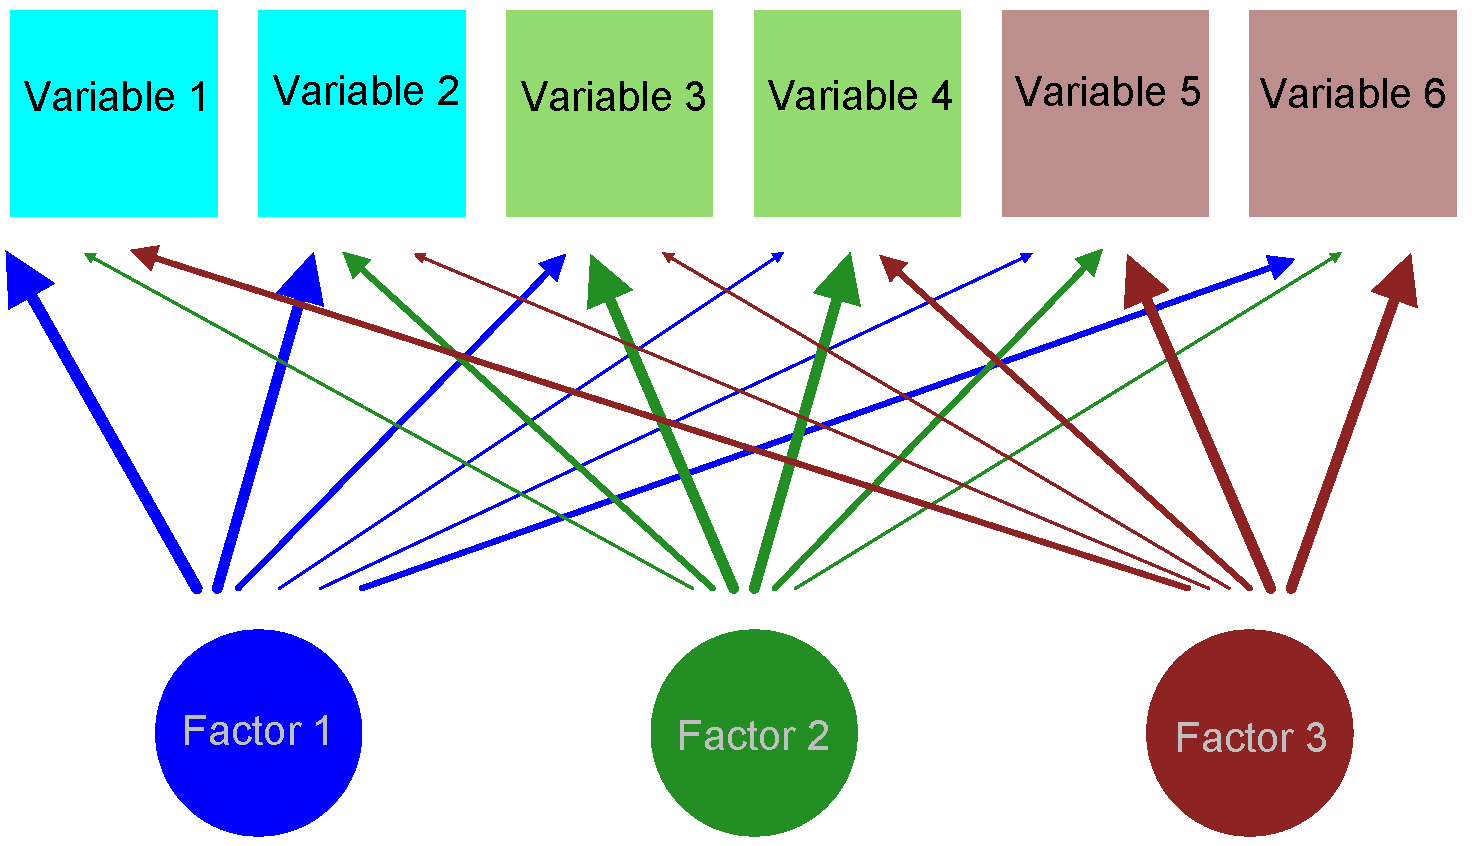
\includegraphics[width=0.75\textwidth]{Graphics/Variable-Factor}
\end{figure}

The following sources may offer additional help: \parencite{Hop-75,Wil-10,Klo-10,Fae-16,Fri-17}. If two observed variables \AbsVec{x, y} are correlated, then a change in a third, underlying (confounding), latent (unobserved) variable (\textbf{factor}) may be the cause (see fig. \ref{fig:VarFac}). Factor analysis is used to uncover such factors from an observed data set:
\begin{equation}
     z_{i,j} = \psi_{i,j} + \sum\limits_{k=1}^p \arr{L}_{j,k} \arr{C}_{i,k}
\end{equation}
with:
\begin{description}
    \item[\( z_{i,j} \)]{result of person \skalar{i} on item \skalar{j}, in standard deviations from mean}
    \item[\( \psi_{i,j} \)]{measurement error of person \skalar{i} on item \skalar{j}}
    \item[\( \arr{L}_{j,k} \)]{loading of factor \skalar{k} on variable \skalar{j}, that is, the correlation of \skalar{\AbsVec{F}_{j,k}} with variable \skalar{j} }
    \item[\( \arr{C}_{i,k} \)]{factor score of student \skalar{i} on factor \skalar{k} (\( \bar{\arr{C}} = 0, \sigma_\arr{C} = 1 \))}
\end{description}
The number of latent factors \skalar{p} is initially equal to the number of observed variables. However, often only a small number \skalar{q} of the factors is significant. The \textbf{eigenvalue} for each factor is the sum of the squared loadings of a factor on all variables. It explains how much of the  variance \skalar{\sigma} in the data is explained by that factor (column sum to the loading matrix). The data are usually \skalar{z}-standardised and hence have a variance of \skalar{1.0}. An eigenvalue of \num{1.0} therefore means that the factor explains as much variance as an observed variable. The ratio of eigenvalues is ratio of explanatory power of two factors. One can therefore use only those factors with significant eigenvalues, the reminder are thought to originate from experimental noise. The \textbf{communalities} \AbsVec{H} are the sum of the squared loadings of a variable over all factors (row sum of the squared loading matrix). It is the proportion of variance of the variable that can be explained by the factors. In the literature one may find the \textbf{uniqueness} instead, which is the 1 -- \AbsVec{H}.

The differences between Factor analysis and principle component analysis are:
\begin{itemize}
  \item{\acs{PCA} produces components, \acs{FA} factors. Components are a linear combination of observed variables, variables are a linear combination of the underlying factors.}
  \item{\acs{PCA} assumes that the data matrix is error free (all diagonal elements of the correlation matrix are unity), the components therefore contain error and are therefore not equal to latent variables (they are not necessarily interpretable). In \acs{FA} the data are assumed to contain error (diagonal elements of the correlation matrix contain communalities), and the factors extracted contain only the common variance (variance shared with other variables), but not the unique variance (variance specific to a particular variable, which is taken as error term). As a result, the correlation matrix is reconstructed by the components, but only approximated by the factors.}
  \item{\acs{PCA} is used to describe empirical data in causal modelling and to reduce the number of dimensions to ease further analysis (\Foreign{e.g.}, by cluster analysis or multidimensional regression). \acs{FA} is used to theoretically explore the underlying factor structure.}
  \item{In fig. \ref{fig:VarFac} the arrows have opposite direction for \acs{PCA}.}
  \item{\acs{PCA} tries to explain as much as possible of the variance of the variables (\( \sum_{i=1}^p{\AbsVec{s}_{ii}} \)) by reducing the elements of \arr{R} near the diagonal. \acs{FA} tries to account for the covariance between variables (\( \sum_{i,j=1}^p{\AbsVec{s}_{ij}}, i \neq j \)) by reducing the elements far from the diagonal. However, since the one cannot be achieved without the other, both methods do in practice nearly the same thing. }
\end{itemize}
The communality is the variance a variable shares with all other variables. With a high enough number of variables and subjects, the method used seems to have little impact on the results obtained (at least if the communalities are \(> 0.4 \)), so \acs{PCA} is the method of choice when there is no specific reason to use another (\parencite{Wil-10}, but see also \parencite{Cos-05} for a different opinion).

\section{Is a data set suitable for factor analysis and \acs{PCA}?}

\subsection{Number of data}

There are several criteria available. As a rule of thumb \parencite{Wil-10}, there should be at least 6, better more (up to 20 has been suggested) subjects per variable, so if 100 variables are studied, 600 subjects are required, 2000 would be ideal. Each factor should have a chance to be represented by several variables, for most studies that means that there should be \(> 30 \) variables.

The sampling density (average distance between data points) is proportional to \(n^\frac{1}{p} \), thus the number of samples \skalar{n} required for a reasonable representation of the data space increases rapidly with \skalar{p}.

\subsection{Correlation coefficients}

Most (off-diagonal) correlation coefficients should be \(0.3 < r < 0.8 \), with around \num{0.5} being ideal.

\subsection{Multivariate normality of data}\label{text:MulNorm}

Both \acs{FA} and \acs{PCA} require that the data are distributed multivariate normal, that is, every linear combination of its \skalar{p} components has a univariate normal distribution (\( ax_{\cdot i} + bx_{\cdot j} \) is normally distributed \(\forall\enspace i,j \in [1\ldots p] \) and \(a,b \in \set{R} \)). \parencite{Zyg-14} recommends the procedures in \parencite{Roy-95} (FORTAN-code available in \parencite{Mil-04}) and \parencite{Hen-90} to test this, both are available in the R-package MVN \parencite{Kor-14}. It is also possible to test for normality of each variable, this must be true if multivariate normality is true. Note, however, that normality of the individual data is necessary but not sufficient for multivariate normality of the entire set (see for example fig. \ref{fig:MultNorm} on page \pageref{fig:MultNorm}).

\subsection{The \Name{Kaiser-Meyer-Olkin} (KMO) criterium}

\begin{table}
  \caption{Interpretation of MSA-values according to \parencite{Kai-74}}
  \label{tab:KMO}
  \centering
    \begin{tabular}{ll}
      \toprule
      KMO        & Suitability \\
      \midrule
 \(> \) 0.90   & marvellous  \\
      0.80..0.90 & meritorious \\
      0.70..0.89 & middling    \\
      0.60..0.69 & mediocre    \\
      0.50..0.59 & miserable   \\
 \(< \) 0.50   & unacceptable\\
      \bottomrule
    \end{tabular}
\end{table}

For a correlation matrix \skalar{r} to be useful for factor analysis, \(\skalar{r}^{-1} \) should be near diagonal.
The KMO-criterium measures how close \(\skalar{r}^{-1} \) is to being diagonal:
\begin{equation}
  \mathrm{KMO} = \frac{\sum_{i=1}^{n}{\sum_{j=1}^{n}{r^2_{ij}}}}{\sum_{i=1}^{n}{\sum_{j=1}^{n}{r^2_{ij}}} +
  \sum_{i=1}^{n}{\sum_{j=1}^{n}{q^2_{ij}}}}, \qquad i \neq j
\end{equation}
with \skalar{r_{ij}} the correlation of variables \skalar{i} and \skalar{j} and \skalar{p_{ij}} the partial
correlation \parencite{Cer-77}:
\begin{align}
  \AbsVec{Q} &= \AbsVec{D} \skalar{r}^{-1} \AbsVec{D} \\
  \AbsVec{D} &= [(\diag{\skalar{r}^{-1}})^{1/2}]^{-1}
\end{align}
A large partial correlation means that the correlation matrix has little common variance and results in a small
KMO-value (see table \ref{tab:KMO}). It is also possible to use the \textbf{measure of sampling adequacy (MSA)} to
determine whether a particular variable \skalar{j} should be included in the analysis:
\begin{equation}
  \mathrm{MSA}_j = \frac{\sum_{i \neq j}{r^2_{ij}}}{\sum_{i \neq j}{r^2_{ij}} + \sum_{i \neq j}{q^2_{ij}}}
\end{equation}
If variables with a poor MSA are removed from the analysis, the overall KMO increases.

However, as shown by \parencite[p. 147]{Ren-02}, MSA is affected not only by the quality of \skalar{r}, but also
decreases with the number of significant factors. It therefore is of limited value.

\subsection{\Name{Bartlett}'s sphere test}

Tests \(H_0: \skalar{r} = \AbsVec{I} \) (the identity matrix) \Foreign{vs} \(H_1: \skalar{r} \neq \AbsVec{I} \)  \parencite{Bar-51}. If \(H_0 \) were true then there is no covariance between data, and the data points form a perfect sphere in \skalar{p}-dimensional space. Then of course there would be no principal component, all eigenvalues are identical except for noise.
\begin{align}
  \chi^2 &\approx -\left[(n-1)-\frac{2p+5}{6}\right] \times \log(||\arr{R}||) \\
  f      &= \frac{p(p-1)}{2}
\end{align}
with \skalar{||\arr{R}||} the determinant of the correlation matrix (which would be unity if \skalar{r} =
\AbsVec{I}). The correlation matrix is suitable if \(P_0 < \SI{5}{\%} \). The test is sensitive to deviation of the
data from multivariate normal distribution, which may lead to false acceptance of \(H_0 \).

\Name{Bartlett}'s test compares the volume of the data ellipsoid with the volume of the spheroid that would result if all axes were identical.  Another way to calculate \(\chi^2 \) is via the ratio between the geometric and arithmetic mean of all eigenvalues of the correlation matrix (which would be unity if the data were spherical):
\begin{align} \label{eqn:Bart}
  r      &= \frac{\tilde{\lambda}}{\bar{\lambda}} = \frac{\sqrt[p-k]{\prod_{i=k+1}^{p}{\lambda_i}}}{\frac{1}{p-k} \sum_{i=k+1}^{p}{\lambda_i}} \\
  \chi^2 &= -(n - (p-k) - 0.5) \times \ln(r^{p-k}) \notag \\
  f      &= \frac{(p - k - 2)(p - k - 1)}{2} \notag
\end{align}
with \skalar{k} the number of eigenvalues excluded from the analysis (in this context 0, but see eqn. \ref{eqn:BartNo}, where this becomes important).

\begin{lstlisting}[caption=\Name{Bartlett}'s sphere test]
  function Bartlett (const Cor : MatrixTyp; Cases : word) : float;

  var f, Variables  : word;
      chi2, Det, P0 : extended;

  begin
    Variables := MatrixRows(Cor);
    Det := Determinante(Cor);
    write('Determinante = ', det:10, ' ');
    chi2 := -(pred(Cases) - (2 * Variables + 5) / 6) * log(Det, 10);
    f := round(Variables * pred(Variables) / 2);
    write('chi2 := ', chi2:5:3, ' ', 'f = ', f:5, ' ');
    P0 := IntegralChi(chi2, f); // should be larger than 0.95
    writeln('P0 = ', (100*P0):3:1, '%');
    Bartlett := P0;
  end;
\end{lstlisting}

\section{Mathematical basis of principle component analysis}

\begin{figure}
   \caption{Geometrical interpretation of PCA, for a two-dimensional variable set. Each attribute carrier is
   represented by a (\emph{red}) dot in the \(\AbsVec{x}_1, \AbsVec{x}_2 \)-plane. All data form an ellipsoid cloud,
   with the ellipsoid representing a surface of identical density. Transformation occurs by centering the
   ellipsoid (subtracting the vector of averages \(\bar{\AbsVec{x}}_1, \bar{\AbsVec{x}}_2, \ldots
   \bar{\AbsVec{x}}_p \), \emph{purple}) and rotating the coordinate system so that the first principal component
   (\emph{green}) is the largest radius of that ellipsoid, the eigenvalue is the length of this vector. The second
   principal component is orthogonal to the first, and represents the second-largest radius of the ellipsoid, and
   so on for higher dimensions. }
   \label{fig:PCA-geo}
   \centering
      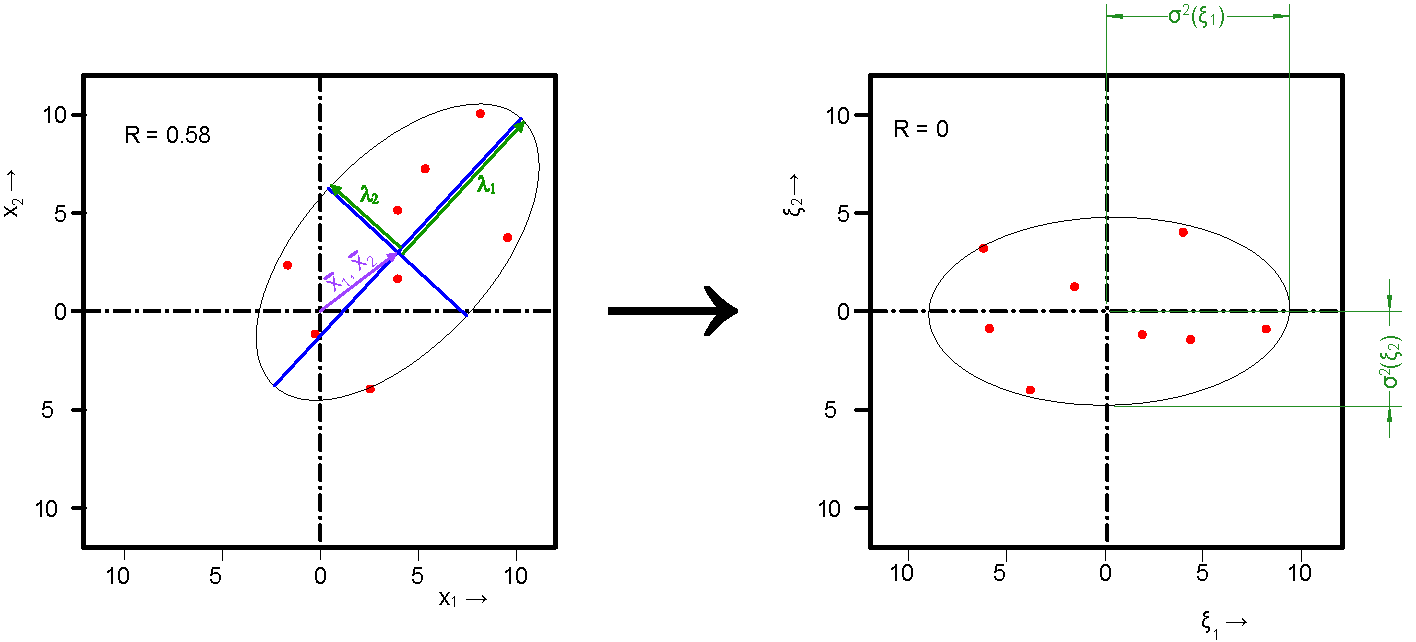
\includegraphics[width=\textwidth]{Graphics/PCA}
\end{figure}

\begin{figure}
   \caption{Distance of a point to the regression line (\emph{green, left}) and the principle component (\textit{purple, right}) for the 2D case. In linear regression, the independent variable \skalar{x} is assumed to be error free, and the distance of a data point to the regression line is measured in the direction of the dependent variable \skalar{y} (orthogonal to the \skalar{x}-axis). In \acs{PCA} all variables are equivalent, measurements for each individual have errors in both \skalar{x}- and \skalar{y}-direction. The distance of the data point to the principle component is orthogonal to that component (as in \Name{Deming}-regression with \(\sigma = 1 \), see section \ref{sec:Deming} on page \pageref{sec:Deming}). }
   \label{fig:DirDist}
   \centering
      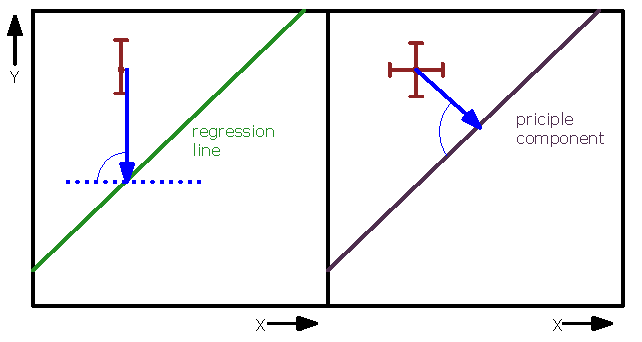
\includegraphics[width=0.75\textwidth]{Graphics/DirectionOfDistance}
\end{figure}

\begin{figure}
   \caption{There is only one direction of the principle axis that maximises the spread of the projection of the data (variance), in this position the distance of the data points from the axis is minimal. Data points in blue, projections in red.  One can think of the distances as springs, which apply a force onto the principle component according to \Name{Hooke}'s law. Then the component will orient itself so that the overall force is zero. Figure from \href{https://stats.stackexchange.com/questions/2691/making-sense-of-principal-component-analysis-eigenvectors-eigenvalues?rq=1}{https://stats.stackexchange.com/questions/2691/making-sense-of-principal-component-analysis-eigenvectors-eigenvalues?rq=1}. }
   \label{fig:MaxVar}
   \centering
   \includemedia[
       label=,
       width=\linewidth,height=0.4\linewidth,
       addresource=AxisRotation.flv,
       transparent, %transparent player background
       activate=pageopen,
       passcontext, %show VPlayer’s rightclick menu
       flashvars={
          source=AxisRotation.flv
          &loop=true
       }
       ]{}{VPlayer.swf}
\end{figure}

PCA was invented by \Name{Hotelling} \parencite{Hot-33}, using the work of several authors. The data in a data matrix \AbsVec{X} can be interpreted as points in a \skalar{p}-dimensional cloud (see fig. \ref{fig:PCA-geo}). The data points are enveloped by an ellipsoid (ellipse in the two-dimensional case), which represents a surface of equal density.

The first principle component is, in effect, a kind of regression line through the data cloud (actually, linear regression minimises the distances from the regression line as measured orthogonal to the \skalar{x}-axis, in \acs{PCA} they are measured orthogonal to the component, see fig. \ref{fig:DirDist}). If we calculate the distance of all data points from the regression line, the second principle component would be a regression through those, and so on. The first component coincides with the major axis of the ellipsoid. This vector has \skalar{p} elements and is called an \emph{eigenvector}. In \Name{Euklid}ian space, the length of a vector is the root of the sum of the squares of the elements (see eqn. \ref{fig:PCA-geo}), this length is called \emph{eigenvalue}.

For the data matrix a variance-covariance matrix \(\arr{S} = \AbsVec{X}^T\AbsVec{X} / (p-1) \) (if the data are z-standardised, otherwise the correlation matrix \(\arr{R} \) is used) is calculated.

Aside: Interconversion of \arr{S} and \arr{R}: \(\skalar{r}_{ij} = \frac{\AbsVec{s}_{ij}}{\AbsVec{s}_i \AbsVec{s}_j} \). Hence if \(\arr{A} = \diag(\AbsVec{s}_1, \AbsVec{s}_2, ... , \AbsVec{s}_p) \) a diagonal matrix of variances, then \(\arr{S} = \arr{A}\arr{R}\arr{A} \) is the variance-covariance matrix and and \(\arr{R} = \arr{A}^{-1} \arr{S} \arr{A}^{-1} \).

The sum of squares for both data vectors in the example is \num{500}. For this purpose the data matrix \(\AbsVec{X}_{n \times p} \) is multiplied with a weight matrix \(\AbsVec{F} \), resulting in a factor score matrix \arr{C}: \(\arr{C} = \AbsVec{X} \AbsVec{F} \). Then the sums of squares (= eigenvalues) are now differently distributed (\num{400} and \num{100} instead of \num{208} and \num{292}, respectively), but their sum is the same. Also, the correlation between \(\AbsVec{c}_1 \) and \(\AbsVec{c}_2 \) is now \num{0}, the components are independent. The eigenvalues are arranged in a diagonal matrix \(\Lambda \):
\begin{gather}
   \Lambda = \begin{pmatrix} \lambda_1 & 0 \\ 0 & \lambda_2 \end{pmatrix} =
  \begin{pmatrix} 400 & 0 \\ 0 & 100 \end{pmatrix}
\end{gather}
\AbsVec{F} represents tests, \arr{C} persons, \(\AbsVec{X} = \arr{C} \AbsVec{F}' \).

How do we get \(\Lambda \)? From the \emph{characteristic equation}:
\begin{equation}
  ||\arr{S} - \lambda_i \arr{I}|| = 0
\end{equation}
with \(||\ || \) the determinant and \arr{I} the identity matrix (all diagonal elements 1, all other elements 0).
Thus, in our example the determinant of:
\begin{gather}
  \begin{pmatrix} 208 & 144 \\ 144 & 292 \end{pmatrix} -\lambda_i
  \begin{pmatrix} 1 & 0 \\ 0 & 1 \end{pmatrix} =
  \begin{pmatrix} 208-\lambda_i & 144-0 \\ 144-0 & 292-\lambda_i \end{pmatrix}
\end{gather}
This leads to
\begin{equation}
  \lambda_i^2 - 500 \lambda_i + \num{40000} = 0
\end{equation}
which, when solved for \(\lambda_i \) gives (\num{400}, \num{100}). For each \(\lambda_i \) we can calculate the
corresponding latent vector \(\AbsVec{f}_i \) from
\begin{equation}
  (\arr{S} - \lambda_i \arr{I}) \AbsVec{f}_i = 0
\end{equation}
which is for \(\AbsVec{l}_1 = 400 \):
\begin{gather}
   \left[ \begin{pmatrix} 208 & 144 \\ 144 & 292 \end{pmatrix} - 400
   \begin{pmatrix} 1 & 0 \\ 0 & 1 \end{pmatrix} \right]
   \begin{pmatrix} 0.6 \\ 0.8 \end{pmatrix}  =
   \begin{pmatrix} -192 & 144 \\ 144 & -108 \end{pmatrix}
   \begin{pmatrix} 0.6 \\ 0.8 \end{pmatrix} =
   \begin{pmatrix} 0 \\ 0 \end{pmatrix}
\end{gather}

Where do the equations
\begin{equation}
  ||\arr{S} - \lambda_i \arr{I}|| = 0 \quad (\arr{S} - \lambda_i \arr{I}) \AbsVec{f}_i = 0
\end{equation}
come from?  If a vector \AbsVec{X} is left-multiplied with an array \arr{A}, another vector \AbsVec{Y} is
obtained, which is called a transformation of \AbsVec{X}: \(\arr{A} \AbsVec{X} = \AbsVec{Y} \). In the case of PCA,
\AbsVec{X} maintains its direction, in our example: \( \arr{S} \AbsVec{F} = \lambda_i \AbsVec{F} \). This is equivalent
to
\begin{equation}
  \arr{S} \AbsVec{F} - \lambda_i \AbsVec{F} = 0 = (\arr{S} - \lambda_i \arr{I}) \AbsVec{F}
\end{equation}
Unless the determinant \(||\arr{S} - \lambda_i \arr{I}|| = 0 \) the vector \(\AbsVec{F} \) will be 0.

Considering fig. \ref{fig:PCA-geo}, there are a few points on the ellipse where the normal of the tangent has the
same direction as the line connecting the point to the focus of the ellipse. This identity determines a latent
vector.

To do a \acs{PCA} perform the following steps:
\begin{enumerate}
  \item{Arrange data in a matrix with persons in rows and variables in columns (\( \AbsVec{X}_{n \times p} \)). }
  \item{Calculate the arithmetic means and standard deviation of all variables of \AbsVec{X} (that is, of all columns).}
  \item{Center the data by subtracting the column means from all columns.}
  \item{From the centered data matrix \arr{X} calculate the variance-covariance matrix \arr{S}, \(\AbsVec{s}_{i,j} = \frac{\sum_{k=1}^{n}{(\AbsVec{x}_{k,i}-\bar{\AbsVec{x}}_i)} \times \sum_{k=1}^{n}{(\AbsVec{x}_{k,j}-\bar{\AbsVec{x}}_j)}}{n-1} \) or the
      correlation matrix \arr{R}. The variance-covariance matrix may also be calculated by \(\arr{S} = \arr{X}^T\arr{X}/(p-1) \), the correlation matrix from \(\arr{R} = \arr{Z}^T\arr{Z} \).}
  \item{Perform an eigenanalysis of either matrix, resulting in the diagonal matrix of eigenvalues \(\Lambda \) and the corresponding eigenvectors (components) \(\arr{E}_{p \times p} \). Note that using \arr{R} or \arr{S} will yield different results unless the data matrix is not only centered, but \skalar{z}-standardised.}
  \item{Calculate the  proportion of explained variance by dividing each eigenvalue \(\lambda_i \) by the sum of
      all eigenvalues \(\sum_{j=1}^p{\lambda_i} = p \), and its cumulative sum.}
  \item{Calculate the acceleration \(f''(j) \approx (f(j+1) - 2f(j) + f(j-1)) \), the second derivative of the scree-plot}
  \item{Calculate the product of the eigenvalues \(\prod_{i=1}^p \lambda_i = ||\arr{R}|| \) required for the sphericity test (see above).}
  \item{Generate the diagonal matrix \skalar{\Lambda} with eigenvalues on the diagonal. This is the variance-covariance of the components. }
  \item{Determine the number of significant eigenvalues \skalar{q}, and keep the corresponding
      eigenvectors in a projection matrix \(\arr{F}_{p \times q} \) column-wise from left to right.}
  \item{Calculate the factor score matrix (principle components) by \(\arr{C}_{n \times q}^T = \arr{X}_{n \times p} \arr{F}_{p \times q} \). }
  \item{Calculate the correlation between variables and factors, the \textbf{loadings} \(\arr{L}_{p \times
      q} \). This is the proportion of variance in a variable that is accounted for by a factor. For each variable, the \textbf{communality}, is calculated as \[\AbsVec{h}_j = \sum_{k=1}^{q}{\AbsVec{l}_{j,k}^2}\], the row sum of squared loadings. Sometimes, in the literature the \textbf{uniqueness}  = \( 1 - \AbsVec{h}_j \) is used instead.}
  \item{Likewise, the column sum of squared loadings is the \textbf{sum of squared loadings}. The SSLoadings divided by its total is \textbf{variance accounted for}. }
  \item{\Name{Hoffman}'s index of complexity \parencite{Hof-77} for each item is \(\frac{(\sum_{k=1}^{q}{l_{jk}^2})^2}{\sum_{j=1}^{q}{l_{j k}^4}} \). }
  \item{If \acs{PCA} is used as a method of factor analysis, identify for each factor the \(\approx \) \num{5} variables that have the highest and lowest correlation and use these to interpret the factors. }
  \item{A rotation of the coordinate system can be tried to obtain more interpretable components. In that case, the scores have to be recalculated to match the rotated loadings. In this case, one should no longer speak of ``principal components'', but of ``rotated components''.}
\end{enumerate}

Asside: \acs{PCA} can also be performed using singular value decomposition on the centered data matrix (\( \arr{X}_{n \times p} = \arr{P}_{n \times p} \Delta_{p \times p} \arr{Q}_{p \times p}^T \)). Columns of  \arr{P} contain the left singular vectors, and \(\arr{F} = \arr{P} \Delta \). These singular vectors are the normalised eigenvectors of \(\arr{X}\arr{X}^T \). Columns of the loading matrix \arr{Q} contain the of right singular vectors, and \arr{X}\arr{Q} gives the projections of data onto the principal components. The vectors in \arr{Q} are the normalised eigenvalues of \(\arr{X}^T \arr{X} \). The diagonal matrix \(\Delta \) contains the singular values and is related to eigenvalues by \(\lambda_i = \delta^2_i \), where \(\Lambda \) contains the eigenvalues of both \(\arr{X}\arr{X}^T \) and \(\arr{X}^T \arr{X} \), which are identical.

The \textbf{non-linear iterative partial least squares (NIPALS)} algorithm calculates the first eigenvector and the first score column of a data matrix, their outer product is subtracted from the data matrix, the resulting residual matrix is used to calculate the second eigenvector/loading vector and so on. With very large data sets (\Foreign{e.g.}, in -omics), which have only a few significant components, this can lead to significant savings in computer time, however, the algorithm is sensitive to roundoff and cancellation errors.

\subsection{Calculation of component and factor scores}

Once the loading matrix \arr{L} has been calculated and -- if desired -- rotated, the next step is the calculation of the scores each individual has on the \skalar{q} relevant factors. As these scores are free of co-linearity, they can be used as variables for further analysis, for example regression or cluster analysis. The dimension of the score matrix \arr{C} is \skalar{n\times q}. For this purpose, a matrix of regression coefficients $\arr{A}_{p\times q}$ is calculated, then  \arr{C} = \arr{XA} or, better, \arr{ZA} if the correlation matrix or the centered values of \arr{X} if the covariance matrix was used. The regression matrix may be saved and used to calculate scores for new observations. The scores calculated have a variance of unity (or nearly so). There are several methods to calculate \arr{A} \parencite{ttn-14}:

\subsubsection{The coarse (\Name{Cattell}'s) method}

\( \arr{A} = \arr{L}\). The data matrix \arr{X} should be centered (if the covariance-matrix \arr{S} was used to calculate \arr{L}) or \skalar{z}-standardised (if \arr{R} was used). It is possible to set low values of \arr{A} to zero, or even to dichotomise all elements of \arr{L} to either zero or unity. The main value of this method used to be that it does not require matrix inversion and hence is computationally cheap, but with the increased power of personal computers that is no longer an issue. Score values also tend to be more stable from sample to sample if sampling is not ideal, the coarse method is hence used mainly in exploratory analysis, where the reliability and validity of the factors has not yet been tested.

\subsubsection{The refined methods}

After unrotated PCA one can simply use \( \arr{A} = \arr{L} \Lambda^{-1} = \arr{R}^{-1} \arr{L} \), that is, each column of \arr{L} is divided (scaled) by the corresponding eigenvalue. The method results in scores that have a variance of unity. If rotation was performed, \( \arr{A} = (\arr{L}^+)^T \), the transposed pseudoinverse.

After factor analysis several methods are available, including:
\begin{description}
  \item[Regression method]{\parencite{Tom-35,Thu-35} \(\arr{A} = \arr{R}^{-1} \arr{LI} \). This formula may also be used in PCA (and is the only method available in SPSS after PCA extraction).}
  \item[\Name{Horst}'s method]{\parencite{Hor-65} \(\arr{A} = \arr{LL}^T\arr{LI} = (\arr{L}^+)^T \). }
  \item[\Name{Anderson-Rubin}'s method]{\(\arr{A} = \arr{L}^T\arr{U}^{-1} \arr{R} \arr{U}^{-1} \arr{L} \). The scores have a variance of exactly one. This method can be used only after orthogonal, not oblique, rotations.}
  \item[\Name{McDonald-Anderson-Rubin}'s method]{\(\arr{A} = \arr{R}^{1/2} \arr{GH}^T \arr{I}^{1/2} \), where \( \svd(\arr{R}^{1/2} \arr{U}^{-1} \arr{L} \arr{I}^{1/2}) = \arr{G}\Delta\arr{H}^T \). This method is an extension of {Anderson-Rubin}'s method that works after both orthogonal and oblique rotations.  }
  \item[\Name{Green}'s method]{is a modification of \Name{McDonald-Anderson-Rubin}'s method, where \( \svd(\arr{R}^{1/2} \arr{L} \arr{I}^{3/2}) = \arr{G}\Delta\arr{H}^T \). This method may also be used after PCA, giving the same result as \Name{Horst}'s.}
\end{description}

\section{Pascal program for PCA}

The main program then is as follows:
\begin{lstlisting}[caption=Main program for PCA]
  PROGRAM Principal;

  USES
    Math,              // Lazarus math UNIT
    mathfunc,          // basic mathematical routines FOR real AND INTEGER
    Complex,           // routines FOR complex numbers
    Vector,            // vector algebra
    Matrix,            // basic matrix algebra
    stat,              // statistical TEST distributions
    Correlations,      // various types OF correlation coefficients
    PCA,               // principal component analysis
    PerformShrinkage,  // Ledoit-Wolf shrinkage OF correlation matrix
    Rotation,          // rotation OF loading matrix
    SystemSolve,       // linear equations
    EigenValues,       // calculation OF eigenvalues
    Zufall;            // generate Random numbers

  VAR
    Types                                                : TypeVector;
    EV, Variance, CumVariance, ImputVector, Acc,
    Communalities, Uniqueness, VarianceAccounted         : VectorTyp;
    Data, Cor, EigenVectoren, Scores, Identity, Loadings : MatrixTyp;
    Freqs                                                : FreqsType;
    x                                                    : float;
    Cases, i, iter                                       : WORD;


  BEGIN
    ProblemName := 'Anonym';
    SigVecs := 40;
    ReadCSV(Types, Data);
    CalculateCorrelationMatrix(Data, Types, Cor);
    WriteCorrelations(Cor, FALSE);
    Cases := MatrixRows(Data);
    Average(Cor, 0.5);               // perform shrinkage by average correlation
    WriteCorrelations(Cor, TRUE);
    AnalyseFrequencies(Cor, Types, Freqs);
    WriteCorrelations(Cor, TRUE);
    x := Bartlett(Cor, Cases);
    i := Jacobi(Cor, EV, EigenVectoren, Iter); // eigenanalysis
    Writeln('Jacobi: ', Iter: 3, ' iterations, Result = ', i:2, ': ', EigenError[i]);
    DestroyMatrix(Cor);
    SortEigenValues(EV, EigenVectoren);
    ExplainedVariance(EV, Acc, Variance, CumVariance);
    WriteEigenVector(EigenVectoren);
    Writeln('Eigenvectors and -values written');
    MaximumLikelihood(Data, Types, ImputVector);       // Scores
    RobustProduct(Data, EigenVectoren, ImputVector, Scores);
    WriteComponentScores(Scores);
    Writeln('scores written');
    CalculateLoadings(Data, Scores, Types, Loadings);  // unrotated Loadings
    CalculateCommunalities(Loadings, Communalities, Uniqueness, VarianceAccounted);
    WriteLoadings(Loadings, Communalities, Uniqueness, VarianceAccounted, FALSE);
    Writeln('Loadings and communalities calculated and written');
    DestroyVector(Variance);
    DestroyVector(CumVariance);
    DestroyVector(Communalities);
    CreateIdentityMatrix(Identity, SigVecs);
    GradProjAlgOrth(Loadings, Identity, Varimax);      // rotation
    CalculateCommunalities(Loadings, Communalities, Uniqueness, VarianceAccounted);
    WriteLoadings(Loadings, Communalities, Uniqueness, VarianceAccounted, TRUE);
    DestroyMatrix(Identity);
    DestroyMatrix(Data);
    DestroyMatrix(EigenVectoren);
    DestroyMatrix(Scores);
    DestroyMatrix(Loadings);
    DestroyVector(EV);
    DestroyVector(ImputVector);
    DestroyVector(Communalities);
    Writeln('All done, press <CR> to finish:');
    ReadLn;
  END.
\end{lstlisting}

The actual beef is in units \texttt{PCA, PerformShrinkage} and \texttt{Rotation}.

\section{Example: Phylogentic trees from nucleic acid sequences}

All life on earth is thought to originate from a single primordial Archaea-like cell that arose about \num{3.5e9} years ago. This common origin is reflected by sequence similarities in the sequences of common genes. More closely related species have more similar sequences than species whose last common ancestor lived long ago. Thus, it is possible to derive the \emph{tree of life} from sequence comparison, this is a task of bioinformatics.

Usually, sequences are compared by aligning them and then counting differences (insertions, delitions, mutations). However, multiple sequence alignment is computationally expensive, the problem is NP-complete. There are heuristic solutions to the problem implemented in programs like \texttt{Clustal} \parencite{Lar-07} or \texttt{MUSCLE} \parencite{Edg-04}.

\begin{figure}
 \caption{\capstart Phylogenetic tree of Corona- and Lentivirus, using nucleic acid word frequencies (word length = \num{4}). The first principal component of that matrix corresponds to the virus family, the second to similarity within a family. These principal components are sufficient to calculate a distance matrix and a hierarchical tree that agrees well with our knowledge of virus evolution. Compared to \texttt{Clustal}, which required almost \SI{4}{h} to calculate a similar tree by multiple sequence alignment, this calculation took only seconds. For details see text.}
   \label{fig:PincComp}
   \centering
     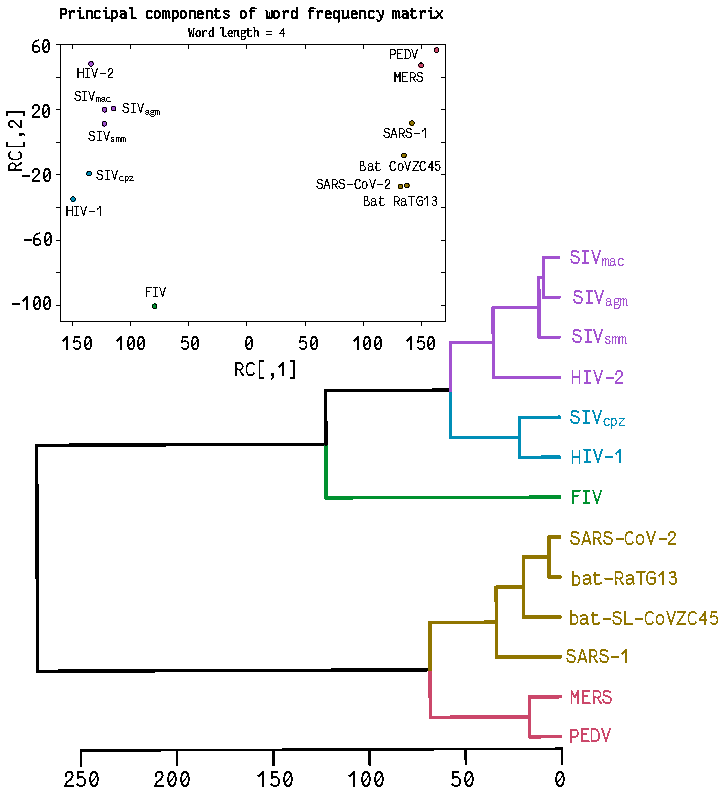
\includegraphics[width=0.75\textwidth]{Graphics/PrincComp}
\end{figure}

It has been shown that a lot of information about a nucleic acid sequence is contained in the word count \parencite{Bas-03,Hac-11}. For example, the sequence ``acg'' contains two words of length two: ``ac'' and ``cg''. Thus, the result of this operation is a 2D data matrix with \skalar{n} rows (\acs{OTU}s) and the possible words (\num{16}, \num{64}, \num{256}, \num{1024}, for word lengths of \num{2}, \num{3}, \num{4}, \num{5}, respectively) in columns. To avoid too many empty cells, word length should be \( < \log_4(m) \), where \skalar{m} is the sequence length. The resulting frequency table can be either used directly to calculate a distance matrix, or subjected to \acs{PCA} first. In the latter case, the first two principal components are sufficient for clustering (see fig. ref{fig:PincComp}).

